\chapter{Evenwichtsconstanten en evenwichtsverschuivingen}\label{ch:b2:equilibrium-shifts}

Een ammoniakfabriek laat haar converter draaien bij ongeveer \qty{450}{\celsius} en
\qty{200}{bar}. Bij kamertemperatuur ligt het evenwicht van \ce{N2 + 3H2 <=>
2NH3} zo ver naar de kant van ammoniak dat een mengsel van de elementen in
principe bijna volledig omgezet kan worden; toch verhitten de ingenieurs het, wat
het evenwicht terugduwt, en comprimeren ze het daarna tot tweehonderd
atmosfeer, wat veel energie kost. De redenen zijn een
compromis tussen hoe ver een reactie kan gaan en hoe snel ze verloopt. Dit
hoofdstuk zet de \omterm{def:b2:reaction-free-energy:gibbs-energy}{gibbsenergie} van de vorige hoofdstukken om in de
evenwichtsconstante van het deel van jaar~1, laat zien hoe die constante verandert
met de temperatuur, telt hoeveel voorwaarden een experimentator vrij
mag kiezen, en voorspelt in welke richting een evenwicht verschuift wanneer de
temperatuur, de druk of de samenstelling verandert.

\begin{recall}
\Cref{ch:b2:reaction-free-energy}: het evolutiecriterium $\Delta_r G\,\dd\xi
\leq 0$ en de betrekking van Gibbs--Helmholtz;
\cref{ch:b2:chemical-potential}: $\Delta_r G = \Delta_r G^\circ + RT\ln Q$.
Het deel van jaar~1: het reactiequotiënt $Q = \prod_i a_i^{\nu_i}$, de
standaardevenwichtsconstante $K^\circ$ als waarde van $Q$ bij evenwicht, de
massawerkingswet en de regel ``$Q < K^\circ$: voorwaarts'', daar alle als
wetten geformuleerd; voortgangstabellen; eindtoestanden van één of twee reacties. Het
beloofde ook dat de keuze van temperatuur en druk voor ammoniak en voor
zwaveltrioxide hier verklaard zou worden.
\end{recall}

\begin{omfigure}
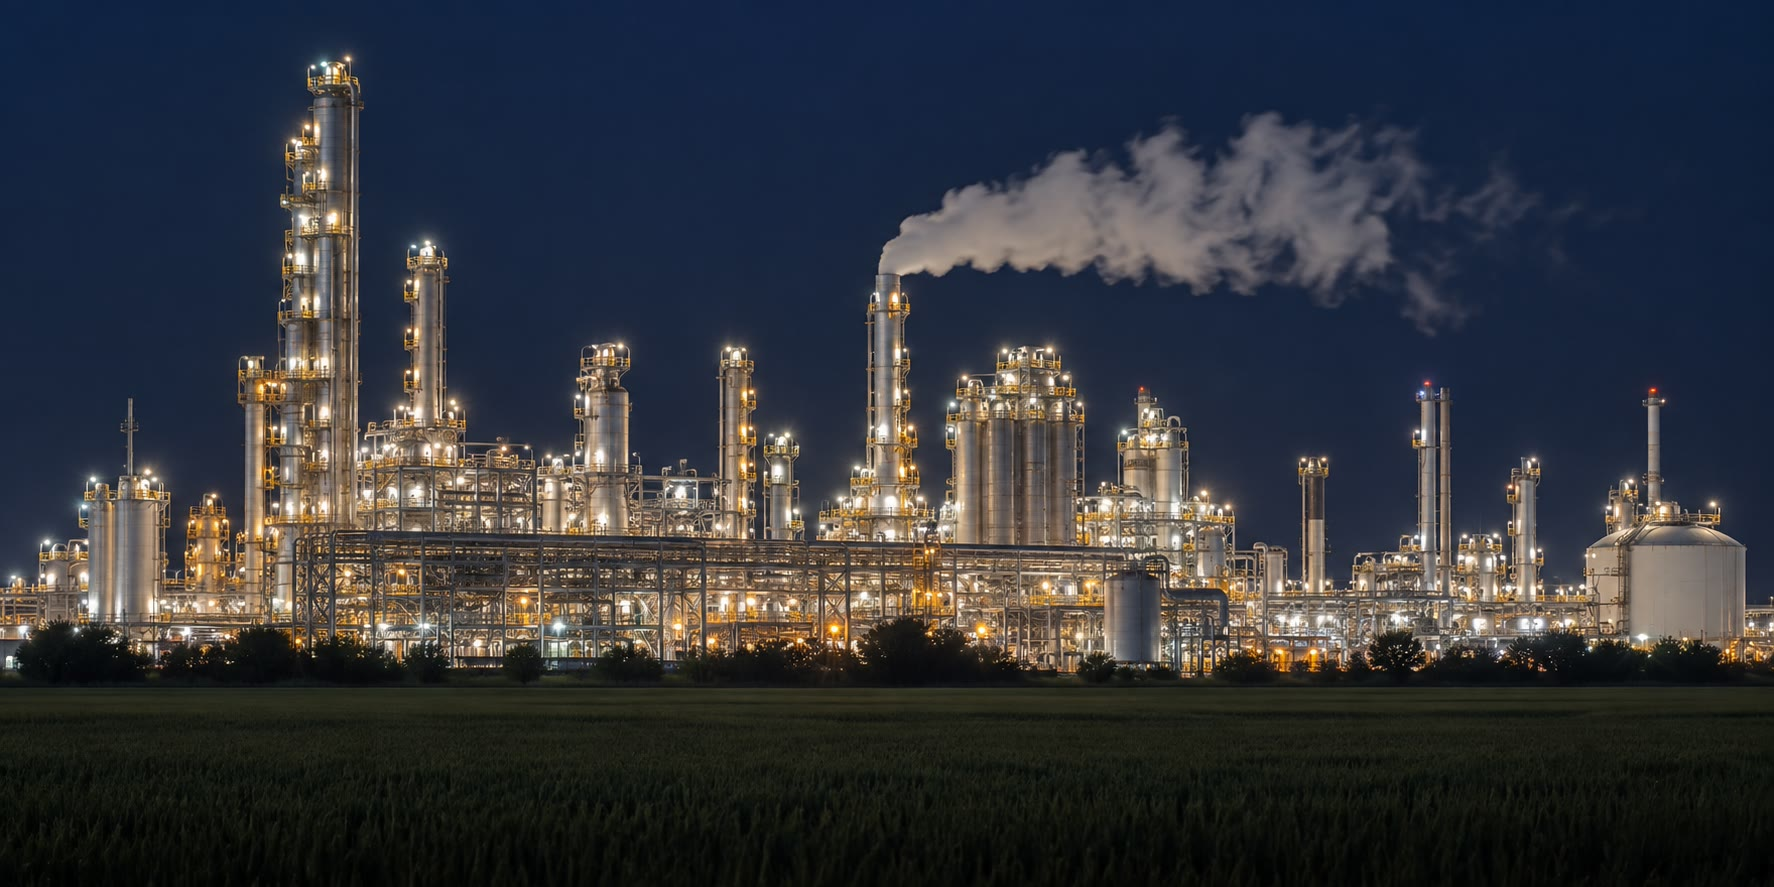
\includegraphics[width=0.7\linewidth]{images/book3/ai/b2-04-ammonia-plant.jpg}

{\small Een ammoniakfabriek bij nacht. In haar converter stromen stikstof en waterstof
over een ijzerkatalysator bij enkele honderden graden en enkele honderden bar;
de keuze van die omstandigheden is het onderwerp van het weekendprobleem.}
\end{omfigure}

\section{De evenwichtsconstante uit de gibbsenergie}

\begin{theorem}[Standaardevenwichtsconstante]\label{thm:b2:equilibrium-shifts:k-from-g}
Bij evenwicht is $\Delta_r G = 0$, en het reactiequotiënt neemt de waarde
\[
  K^\circ(T) = \exp\!\left(-\frac{\Delta_r G^\circ(T)}{RT}\right), \qquad
  \Delta_r G^\circ(T) = -RT\ln K^\circ(T) .
\]
aan. Ze hangt alleen van de temperatuur af.
\end{theorem}

\begin{proof}
Het evolutiecriterium maakt $\Delta_r G = 0$ tot de evenwichtsvoorwaarde.
Met $\Delta_r G = \Delta_r G^\circ + RT\ln Q$
(\cref{prop:b2:chemical-potential:delta-g-q}) betekent evenwicht $\ln Q_{\text{eq}}
= -\Delta_r G^\circ/(RT)$, een functie van alleen $T$, omdat $\Delta_r G^\circ$ dat is.
\end{proof}

\begin{corollary}[De wetten van het deel van jaar~1]\label{cor:b2:equilibrium-shifts:mass-action}
$\Delta_r G = RT\ln(Q/K^\circ)$. Een systeem met $Q < K^\circ$ evolueert dus
voorwaarts, een met $Q > K^\circ$ achterwaarts, en een met $Q = K^\circ$ is in
evenwicht (de massawerkingswet).
\end{corollary}

\begin{proof}
Substitueer $\Delta_r G^\circ = -RT\ln K^\circ$ in $\Delta_r G = \Delta_r G^\circ
+ RT\ln Q$; het teken van $\Delta_r G$ is dat van $\ln(Q/K^\circ)$, en het
evolutiecriterium vereist $\Delta_r G\,\dd\xi \leq 0$.
\end{proof}

\begin{example}[Drie constanten bij \qty{298}{K}]\label{ex:b2:equilibrium-shifts:constants}
Ammoniaksynthese, $\Delta_r G^\circ = \qty{-32.8}{kJ/mol}$: $K^\circ =
\exp(32\,800/(8.314 \times 298.15)) = \num{5.6e5}$ (de tabellen, met meer
cijfers, geven \num{5.4e5}). De dissociatie van \ce{N2O4}, $\Delta_r G^\circ =
\qty{+4.7}{kJ/mol}$: $K^\circ = 0.15$. De ontleding van kalksteen,
$\Delta_r G^\circ = \qty{+130.4}{kJ/mol}$: $K^\circ = \num{1.5e-23}$, en de
evenwichtsdruk van koolstofdioxide boven kalksteen bij kamertemperatuur
is $\num{1.5e-23}$ bar, helemaal niets. Een verandering van \qty{5.7}{kJ/mol} in
$\Delta_r G^\circ$ bij \qty{298}{K} vermenigvuldigt of deelt $K^\circ$ door tien.
% ledger: dfh:NH3_g, s0:NH3_g, janafG:NH3.298.15 (computed in figdata/bachelor-2/thermo-data.py and vant-hoff.py)
\end{example}

De \omterm{def:b2:reaction-free-energy:gibbs-energy}{gibbsenergie} van het hele systeem laat hetzelfde zien als een landschap:
ze is minimaal bij de evenwichtsvoortgang, waar haar helling, $\Delta_r G$,
nul is.

\begin{omfigure}
\begin{tikzpicture}
\begin{axis}[
  width=0.7\linewidth, height=5.6cm, xmin=0, xmax=1, ymin=-2.2, ymax=5.2,
  axis x line=bottom, axis y line=left, xlabel={voortgang $\xi$ (mol)},
  ylabel={$G(\xi) - G(0)$ (\unit{kJ})},
  tick label style={font=\small}, label style={font=\small}, clip=false]
\addplot[omDef, very thick] table[x=xi, y=G] {figdata/out/bachelor-2-gibbs-extent.dat};
\draw[dotted] (axis cs:0.189,-2.2) -- (axis cs:0.189,-0.949);
\fill[omThm] (axis cs:0.189,-0.949) circle (1.6pt);
\node[omThm, anchor=west, font=\small] at (axis cs:0.21,-1.75) {evenwicht, $\xi = 0.189$};
\draw[dashed, gray] (axis cs:0,0) -- (axis cs:1,4.728);
\node[gray, font=\scriptsize, anchor=south east] at (axis cs:1,4.75) {$\xi\,\Delta_r G^\circ$};
\end{axis}
\end{tikzpicture}

{\small \omterm{def:b2:reaction-free-energy:gibbs-energy}{Gibbsenergie} van een gesloten systeem van ideale gassen bij \qty{298}{K} en
\qty{1}{bar}, uitgaande van \qty{1}{mol} \ce{N2O4}, als functie van de voortgang van
\ce{N2O4 <=> 2NO2}. Hoewel $\Delta_r G^\circ > 0$ (gestreepte lijn, zuivere
deeltjes), verlaagt het mengen van de twee gassen $G$, en het minimum ligt bij $\xi =
0.189$, waar $Q = K^\circ = 0.15$. Links ervan is de helling $\Delta_r G =
\partial G/\partial\xi$ negatief, rechts ervan positief.}
% ledger: dfh:N2O4_g, s0:N2O4_g, dfh:NO2_g, s0:NO2_g (computed in figdata/bachelor-2/gibbs-extent.py)
\end{omfigure}

\section{Temperatuur: de vergelijking van Van 't Hoff}

\begin{theorem}[Vergelijking van Van 't Hoff]\label{thm:b2:equilibrium-shifts:vant-hoff}
\[
  \frac{\dd\ln K^\circ}{\dd T} = \frac{\Delta_r H^\circ(T)}{RT^2}
\]
(de \emph{vergelijking van Van 't Hoff}\index{vergelijking van Van 't Hoff}): de evenwichtsconstante
van een \omterm{def:b2:reaction-enthalpy:exothermic}{endotherme} reactie neemt toe met de temperatuur, die van
een \omterm{def:b2:reaction-enthalpy:exothermic}{exotherme} reactie neemt af.
\end{theorem}

\begin{proof}
Schrijf $\ln K^\circ = -\Delta_r G^\circ/(RT)$ en gebruik de betrekking van Gibbs--Helmholtz
van \cref{prop:b2:reaction-free-energy:gibbs-helmholtz},
\[
  \frac{\dd}{\dd T}\left(\frac{\Delta_r G^\circ}{T}\right) =
  -\frac{\Delta_r H^\circ}{T^2} ;
\]
en deel door $-R$.
\end{proof}

\begin{proposition}[Geïntegreerde vorm]\label{prop:b2:equilibrium-shifts:integrated}
Als $\Delta_r H^\circ$ constant is tussen $T_1$ en $T_2$ (\omterm{def:b2:reaction-free-energy:ellingham-approximation}{benadering van
Ellingham}), geldt
\[
  \ln\frac{K^\circ(T_2)}{K^\circ(T_1)} = -\frac{\Delta_r H^\circ}{R}\left(
  \frac{1}{T_2} - \frac{1}{T_1}\right),
\]
en $\ln K^\circ$ is een rechte met helling $-\Delta_r H^\circ/R$ als functie van
$1/T$.
\end{proposition}

\begin{proof}
Integreer $\dd\ln K^\circ = (\Delta_r H^\circ/R)\,\dd T/T^2$, waarbij
$\dd T/T^2 = -\dd(1/T)$.
\end{proof}

\begin{omfigure}
\begin{tikzpicture}
\begin{axis}[
  width=0.72\linewidth, height=5.8cm, xmin=0.9, xmax=3.5, ymin=-19, ymax=15,
  axis x line=bottom, axis y line=left, xlabel={$1000/T$ (\unit{1/K})},
  ylabel={$\ln K^\circ$}, tick label style={font=\small},
  label style={font=\small}, clip=false]
\addplot[omThm, dashed, thick] table[x=invT, y=lnK] {figdata/out/bachelor-2-vant-hoff-a-line.dat};
\addplot[omDef, only marks, mark=*, mark size=1.8pt] table[x=invT, y=lnK] {figdata/out/bachelor-2-vant-hoff-a.dat};
\node[omDef, font=\scriptsize, anchor=west] at (axis cs:3.36,13.2) {\qty{298}{K}};
\node[omDef, font=\scriptsize, anchor=north west] at (axis cs:1.03,-15.3) {\qty{1000}{K}};
\node[omThm, font=\small, anchor=south east, align=right] at (axis cs:2.4,8) {helling $-\Delta_r H^\circ(298)/R$\\ $= +11\,050$ K};
\end{axis}
\end{tikzpicture}

{\small De constante van \ce{N2 + 3H2 <=> 2NH3} volgens de tabellen (punten, 298 tot
\qty{1000}{K}) en de rechte van Van 't Hoff, getekend met $\Delta_r H^\circ$ bij
\qty{298}{K} (gestreept). De reactie is \omterm{def:b2:reaction-enthalpy:exothermic}{exotherm}: $K^\circ$ daalt van
\num{5e5} tot \num{3e-7}. Bij hoge temperatuur vallen de punten onder de rechte:
$\Delta_r H^\circ$ wordt negatiever naarmate $T$ stijgt
(\cref{ex:b2:reaction-enthalpy:kirchhoff}).}
% ledger: janafG:NH3.298.15, janafG:NH3.400, janafG:NH3.500, janafG:NH3.600, janafG:NH3.700, janafG:NH3.800, janafG:NH3.900, janafG:NH3.1000, dfh:NH3_g (computed in figdata/bachelor-2/vant-hoff.py)
\end{omfigure}

\begin{method}[Een evenwichtsconstante bij een andere temperatuur]\label{met:b2:equilibrium-shifts:k-at-t}
\begin{enumerate}
  \item Bereken uit de tabellen bij \qty{298}{K} $\Delta_r H^\circ$, $\Delta_r
        S^\circ$ en $K^\circ(298)$.
  \item Gebruik ofwel de geïntegreerde \omterm{thm:b2:equilibrium-shifts:vant-hoff}{vergelijking van Van 't Hoff}, ofwel bereken
        $\Delta_r G^\circ(T) = \Delta_r H^\circ - T\Delta_r S^\circ$ en daarna
        $K^\circ(T)$: beide zijn dezelfde benadering.
  \item Neem voor een breed interval of een grote $\Delta_r C_p^\circ$ liever getabelleerde
        $\Delta_f G^\circ(T)$; een fout van \qty{5.7}{kJ/mol} bij \qty{298}{K}
        (of \qty{13}{kJ/mol} bij \qty{700}{K}) is een factor tien op $K^\circ$.
\end{enumerate}
\end{method}

\begin{history}[Jacobus Henricus van 't Hoff]
\begin{minipage}[t]{0.2\linewidth}\vspace{0pt}
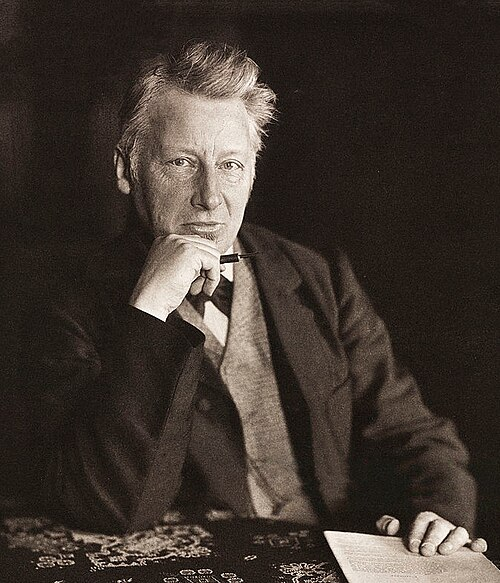
\includegraphics[width=\linewidth]{images/book3/vanthoff.jpg}
\end{minipage}\hfill
\begin{minipage}[t]{0.76\linewidth}\vspace{0pt}
Jacobus Henricus van 't Hoff (1852--1911) gaf in 1884, in zijn
\emph{Études de dynamique chimique}, het verband tussen de temperatuur en
de evenwichtsconstante dat zijn naam draagt, en het jaar daarna de wet van de
\omterm{def:b2:chemical-potential:osmotic-pressure}{osmotische druk} van \cref{ch:b2:chemical-potential}; tien jaar eerder had hij
het tetraëdrische koolstofatoom voorgesteld. Hij kreeg de eerste Nobelprijs voor
Scheikunde, in 1901. (Foto door N. Perscheid, 1904: publiek domein,
Wikimedia Commons.)
\end{minipage}
\end{history}

\section{Variantie}

Hoeveel intensieve grootheden kan een experimentator vrij vastleggen voordat de
evenwichtstoestand volledig bepaald is?

\begin{definition}[Variantie]\label{def:b2:equilibrium-shifts:variance}
De \emph{onafhankelijke intensieve parameters}\index{onafhankelijke intensieve parameter}
van een systeem in evenwicht zijn een verzameling intensieve grootheden
(temperatuur, druk, molfracties in elke fase) die onafhankelijk gekozen
kunnen worden en die, eenmaal gekozen, alle andere vastleggen. Hun aantal is de
\emph{variantie}\index{variantie} $v$ van het systeem.
\end{definition}

\begin{theorem}[Faseregel]\label{thm:b2:equilibrium-shifts:phase-rule}
Voor een systeem van $n$ deeltjes verdeeld over $\varphi$ fasen, verbonden door $r$
onafhankelijke evenwichtsreacties en $s$ bijkomende betrekkingen tussen
intensieve grootheden die door de bereiding vastliggen (een stoichiometrische voeding,
elektroneutraliteit), geldt
\[
  v = c + 2 - \varphi, \qquad c = n - r - s .
\]
\end{theorem}

\begin{proof}
Intensieve variabelen: $T$, $p$, en in elke fase de molfracties van de
$n$ deeltjes, die samen 1 zijn, dus $n - 1$ vrije per fase: in totaal $2 +
\varphi(n - 1)$. Betrekkingen: elk deeltje is in evenwicht tussen de
fasen, $\varphi - 1$ gelijkheden van \omterm{def:b2:chemical-potential:chemical-potential}{chemische potentialen} per deeltje, $n(\varphi -
1)$ in totaal; elke reactie geeft $Q = K^\circ(T)$, $r$ betrekkingen; en $s$
bijkomende betrekkingen. Aftrekken: $v = 2 + \varphi(n - 1) - n(\varphi - 1) - r -
s = n - r - s + 2 - \varphi$. (Een deeltje dat in een fase ontbreekt, verwijdert
tegelijk één variabele en één betrekking.)
\end{proof}

\begin{method}[Een variantie berekenen]\label{met:b2:equilibrium-shifts:variance}
\begin{enumerate}
  \item Som de deeltjes op, met hun fase, en tel $n$ en $\varphi$
        (elke zuivere vaste stof is een fase; alle gassen samen vormen één fase).
  \item Tel de onafhankelijke reacties $r$ ertussen.
  \item Tel de extra betrekkingen $s$: hoeveelheden in stoichiometrische verhouding
        (alleen als de betrekking grootheden van dezelfde fase verbindt),
        elektroneutraliteit van een ionaire oplossing.
  \item $v = n - r - s + 2 - \varphi$.
\end{enumerate}
\end{method}

\begin{example}[Drie varianties]\label{ex:b2:equilibrium-shifts:variances}
Kalksteen in een gesloten vat, \ce{CaCO3(s) <=> CaO(s) + CO2(g)}: $n = 3$, $r =
1$, $\varphi = 3$ (twee vaste stoffen, één gas): $v = 1$. Kies $T$, en de druk
van koolstofdioxide ligt vast: $p = K^\circ(T)\,p^\circ$. Een gasmengsel van
\ce{N2}, \ce{H2} en \ce{NH3} in evenwicht: $n = 3$, $r = 1$, $\varphi = 1$, $v
= 3$ ($T$, $p$ en één samenstellingsvariabele); gemaakt uit ammoniak alleen, of uit
een stoichiometrische voeding, staan \ce{N2} en \ce{H2} in de verhouding 1 : 3, is $s = 1$ en
$v = 2$: bij gegeven $T$ en $p$ ligt de samenstelling vast, zoals het weekendprobleem
gebruikt.
\end{example}

\section{Een evenwicht verschuiven}

\begin{definition}[Verschuiving van een evenwicht]\label{def:b2:equilibrium-shifts:shift}
Wanneer een systeem in evenwicht verstoord wordt (een verandering van temperatuur, van
druk, of van een hoeveelheid), is het in het algemeen niet meer in evenwicht en
evolueert het naar een nieuw evenwicht. De \emph{evenwichtsverschuiving}\index{evenwichtsverschuiving}
is voorwaarts als de reactie voortschrijdt ($\dd\xi > 0$), en anders
achterwaarts.
\end{definition}

\begin{method}[Een verschuiving voorspellen]\label{met:b2:equilibrium-shifts:predict-shift}
Bereken net na de verstoring $Q$ en $K^\circ$ (of schat het teken van hun verandering).
Als nu $Q < K^\circ$, is de verschuiving voorwaarts; als $Q > K^\circ$,
achterwaarts; als de gelijkheid nog geldt, is er geen verschuiving.
\end{method}

\begin{omfigure}
\begin{tikzpicture}[font=\small, >={Stealth}]
  \draw[->, thick] (0,0) -- (11,0) node[right] {$\ln Q$};
  \draw[omThm, thick] (5.5,0.25) -- (5.5,-0.25) node[below, align=center] {$\ln K^\circ$\\ ($= \ln Q$ ervoor)};
  \fill (5.5,0) circle (2pt);
  \draw[omDef, thick] (2.8,0.25) -- (2.8,-0.25) node[below] {$\ln Q$ net erna};
  \draw[->, omDef, very thick] (3.0,0.6) -- (5.2,0.6) node[midway, above] {voorwaartse verschuiving};
  \draw[omProp, thick] (8.4,0.25) -- (8.4,-0.25) node[below] {$\ln Q$ net erna};
  \draw[->, omProp, very thick] (8.2,0.6) -- (5.8,0.6) node[midway, above] {achterwaartse verschuiving};
\end{tikzpicture}

{\small Een verstoring verplaatst $Q$ (of $K^\circ$, als de temperatuur verandert);
het systeem verschuift dan tot opnieuw $Q = K^\circ$: voorwaarts als $Q$
te klein geworden is, achterwaarts als het te groot is.}
\end{omfigure}

\begin{proposition}[Temperatuur]\label{prop:b2:equilibrium-shifts:temperature}
Bij constante druk verschuift een temperatuurverhoging een evenwicht in de
\omterm{def:b2:reaction-enthalpy:exothermic}{endotherme} richting (voorwaarts als $\Delta_r H^\circ > 0$), een temperatuurverlaging in de
\omterm{def:b2:reaction-enthalpy:exothermic}{exotherme} richting.
\end{proposition}

\begin{proof}
Bij vaste samenstelling en druk verandert $Q$ niet met $T$ (voor ideale
systemen); volgens Van 't Hoff neemt $K^\circ$ toe met $T$ als $\Delta_r H^\circ >
0$. Net na een stijging van $T$ is dan $Q < K^\circ$: voorwaarts.
\end{proof}

\begin{proposition}[Druk]\label{prop:b2:equilibrium-shifts:pressure}
Bij constante temperatuur en samenstelling verschuift een verhoging van de totale druk een
evenwicht in de gasfase in de richting die het aantal gasmoleculen
verlaagt ($\Delta\nu_{\text{gas}} < 0$: voorwaarts). Als $\Delta\nu_{\text{gas}}
= 0$, heeft de druk geen invloed.
\end{proposition}

\begin{proof}
Met $p_i = x_ip$ is $Q = \prod_i x_i^{\nu_i}\,(p/p^\circ)^{\Delta\nu_{\text{gas}}}$:
bij vaste samenstelling vermenigvuldigt een verhoging van $p$ het quotiënt $Q$ met
$(p'/p)^{\Delta\nu_{\text{gas}}}$, wat $< 1$ is als $\Delta\nu_{\text{gas}} <
0$. Dan is $Q < K^\circ$: voorwaarts. Gecondenseerde fasen dragen niets bij.
\end{proof}

\begin{proposition}[Een bestanddeel of een inert gas toevoegen]\label{prop:b2:equilibrium-shifts:adding}
Het toevoegen van een kleine hoeveelheid van een gasvormig bestanddeel $j$ aan een evenwicht in de gasfase
verandert $\ln Q$ met
\[
  \left(\frac{\partial\ln Q}{\partial n_j}\right) = \frac{\nu_j}{n_j} -
  \frac{\Delta\nu_{\text{gas}}}{n_{\text{tot}}}\ \ \text{bij constante } T, p ;
  \qquad \frac{\nu_j}{n_j}\ \ \text{bij constante } T, V .
\]
Een inert gas toevoegen heeft geen invloed bij constant volume, en werkt bij constante druk
als een verlaging van de druk.
\end{proposition}

\begin{proof}
Bij constante $T$, $p$: $Q = \prod_i n_i^{\nu_i}\,(p/(p^\circ n_{\text{tot}}))^{
\Delta\nu_{\text{gas}}}$, waarvan de logaritmische afgeleide naar $n_j$ gelijk is aan
$\nu_j/n_j - \Delta\nu_{\text{gas}}/n_{\text{tot}}$ (eerste term nul voor een inert
gas, $\nu_j = 0$). Bij constante $T$, $V$: $p_i = n_iRT/V$ en $Q = \prod_i n_i^{
\nu_i}\,(RT/(p^\circ V))^{\Delta\nu_{\text{gas}}}$, waarvan de afgeleide alleen
$\nu_j/n_j$ is.
\end{proof}

\begin{remark}[Een toegevoegde beginstof die de reactie terugdrijft]\label{rem:b2:equilibrium-shifts:paradox}
Bij de ammoniaksynthese is $\nu(\ce{N2}) = -1$ en $\Delta\nu_{\text{gas}} = -2$:
stikstof toevoegen bij constante $T$ en $p$ verandert $\ln Q$ met $-1/n_{\ce{N2}} +
2/n_{\text{tot}}$, wat positief is wanneer $x(\ce{N2}) > 1/2$. In een mengsel
dat al rijk is aan stikstof verdunt extra stikstof de waterstof zozeer
dat ammoniak ontleedt. De regel ``een beginstof toevoegen duwt voorwaarts'' is betrouwbaar
bij constant volume, niet altijd bij constante druk.
\end{remark}

\begin{proposition}[Principe van Le Chatelier]\label{prop:b2:equilibrium-shifts:le-chatelier}
De bovenstaande eigenschappen worden samengevat door het \emph{principe van Le
Chatelier}\index{principe van Le Chatelier}: een systeem in evenwicht
dat in temperatuur of druk verstoord wordt, verschuift in de richting die
de verstoring tegenwerkt (het neemt warmte op wanneer het verwarmd wordt, verkleint zijn gasvolume wanneer het
samengeperst wordt).
\end{proposition}

\begin{proof}
Het herformuleert \cref{prop:b2:equilibrium-shifts:temperature} (de \omterm{def:b2:reaction-enthalpy:exothermic}{endotherme}
richting neemt warmte op) en \cref{prop:b2:equilibrium-shifts:pressure} (minder
gasmoleculen nemen minder volume in bij dezelfde $T$ en $p$). Voor toevoegingen van
materie bij constante druk is het principe niet betrouwbaar
(\cref{rem:b2:equilibrium-shifts:paradox}): bereken $Q$.
\end{proof}

\begin{remark}[Wanneer het evenwicht verbroken wordt]\label{rem:b2:equilibrium-shifts:rupture}
Een verschuiving kan eindigen, niet in een nieuw evenwicht, maar in het verdwijnen van een fase.
Verhit in een gesloten vat ontleedt kalksteen tot $p(\ce{CO2}) =
K^\circ(T)\,p^\circ$; is er niet genoeg van om die druk te bereiken, dan
verdwijnt hij volledig en blijft $Q$ onder $K^\circ$: het systeem is definitief uit
evenwicht, zoals het deel van jaar~1 al opmerkte.
\end{remark}

\begin{history}[Henry Le Chatelier]
\begin{minipage}[t]{0.2\linewidth}\vspace{0pt}
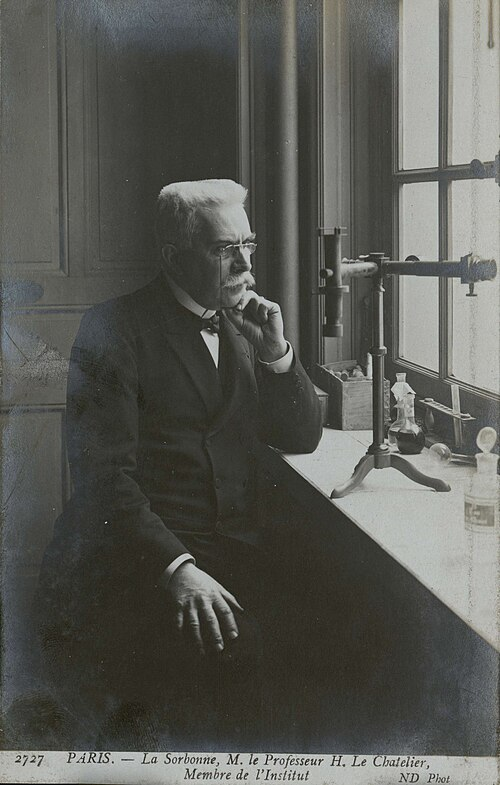
\includegraphics[width=\linewidth]{images/book3/lechatelier.jpg}
\end{minipage}\hfill
\begin{minipage}[t]{0.76\linewidth}\vspace{0pt}
Henry Le Chatelier (1850--1936), mijningenieur en chemicus die werkte aan
cement, metallurgie en pyrometrie, formuleerde in 1884 de ``wet van de verschuiving
van het evenwicht'' die zijn naam draagt. Hij had rond 1901 ook geprobeerd
ammoniak onder druk uit zijn elementen te maken; een explosie in zijn apparatuur maakte
een einde aan die poging. (Foto: onbekende auteur, CC BY-SA 4.0, Wikimedia Commons.)
\end{minipage}
\end{history}

\section{Een synthese optimaliseren}

\subsection*{Ammoniak}

\begin{omfigure}
\begin{tikzpicture}
\begin{axis}[
  width=0.78\linewidth, height=6.2cm, xmin=500, xmax=1000, ymin=0, ymax=0.9,
  axis x line=bottom, axis y line=left, xlabel={$T$ (K)},
  ylabel={molfractie \ce{NH3} bij evenwicht},
  tick label style={font=\small}, label style={font=\small}, clip=false]
\addplot[omThm, very thick] table[x=T, y=p300] {figdata/out/bachelor-2-vant-hoff-b.dat};
\addplot[omDef, very thick] table[x=T, y=p200] {figdata/out/bachelor-2-vant-hoff-b.dat};
\addplot[omProp, very thick] table[x=T, y=p50] {figdata/out/bachelor-2-vant-hoff-b.dat};
\addplot[black!60, very thick] table[x=T, y=p1] {figdata/out/bachelor-2-vant-hoff-b.dat};
\node[omThm, font=\scriptsize, anchor=south west] at (axis cs:600,0.70) {300 bar};
\node[omDef, font=\scriptsize, anchor=north east] at (axis cs:612,0.52) {200 bar};
\node[omProp, font=\scriptsize, anchor=north east] at (axis cs:578,0.30) {50 bar};
\node[black!60, font=\scriptsize, anchor=south west] (onebar) at (axis cs:520,0.13) {1 bar};
\draw[black!60] (onebar.south west) -- (axis cs:512,0.075);
\draw[dotted] (axis cs:723,0) -- (axis cs:723,0.253);
\fill[omDef] (axis cs:723,0.253) circle (1.6pt);
\end{axis}
\end{tikzpicture}

{\small Molfractie ammoniak bij evenwicht uit een 1 : 3-mengsel van stikstof
en waterstof (ideale gassen), als functie van de temperatuur bij vier drukken,
berekend uit de getabelleerde gibbsenergieën. Druk verhoogt haar, temperatuur
verlaagt haar; het punt markeert \qty{723}{K} en \qty{200}{bar}.}
% ledger: janafG:NH3.500, janafG:NH3.600, janafG:NH3.700, janafG:NH3.800, janafG:NH3.900, janafG:NH3.1000 (computed in figdata/bachelor-2/vant-hoff.py)
\end{omfigure}

De synthese is \omterm{def:b2:reaction-enthalpy:exothermic}{exotherm} en brengt vier gasmoleculen terug tot twee: volgens
de bovenstaande eigenschappen begunstigen een lage temperatuur en een hoge druk ammoniak.
Bij \qty{1}{bar} en kamertemperatuur is het evenwicht bijna volledig, maar
de reactie verloopt helemaal niet: de drievoudige binding van stikstof wordt alleen
op een katalysator verbroken, en de ijzerkatalysator werkt pas bij enkele honderden
graden. Fabrieken kiezen daarom:
\begin{itemize}
  \item een temperatuur die hoog genoeg is voor de snelheid, zo laag als de katalysator toelaat
        (rond \qty{700}{K});
  \item een hoge druk om het rendement terug te winnen dat door de temperatuur verloren gaat, begrensd
        door de kosten van compressie en van dikwandige vaten;
  \item een kringloop: het gas dat de converter verlaat, wordt afgekoeld, de ammoniak condenseert
        en wordt afgevoerd, en het niet-omgezette gas wordt met verse voeding teruggevoerd;
        een kleine \omterm{def:b2:equilibrium-shifts:single-pass}{spuistroom} verwijdert het argon en het methaan die zich anders
        zouden ophopen.
\end{itemize}

\begin{definition}[Conversie per doorgang, recyclestroom, spuistroom]\label{def:b2:equilibrium-shifts:single-pass}
In een proces met recyclage is de \emph{conversie per doorgang}\index{conversie per doorgang}
de fractie van een beginstof die bij één doorgang door
de reactor wordt omgezet; het niet-omgezette deel, gescheiden van het product, wordt
als \emph{recyclestroom}\index{recyclestroom} naar de reactorinlaat teruggevoerd; een
\emph{spuistroom}\index{spuistroom} is een kleine stroom die continu uit de
recyclestroom wordt afgetapt om te verhinderen dat inerte deeltjes zich ophopen.
\end{definition}

\begin{omfigure}
\begin{tikzpicture}[font=\small, >={Stealth}, box/.style={draw, thick, rounded corners=2pt, minimum width=2.1cm, minimum height=1.0cm, align=center, fill=white}]
  \node[box] (comp) at (0,0) {compressor};
  \node[box] (conv) at (3.6,0) {converter\\ (katalysator)};
  \node[box] (cond) at (7.2,0) {koeler en\\ scheider};
  \draw[->, thick] (-3.9,0) -- (comp) node[pos=0.0, above right] {verse \ce{N2 + 3H2}};
  \draw[->, thick] (comp) -- (conv);
  \draw[->, thick] (conv) -- (cond);
  \draw[->, thick, omDef] (cond.south) -- ++(0,-1.0) node[below] {vloeibare ammoniak};
  \draw[->, thick, omThm] (cond.north) -- ++(0,0.9) -| (comp.north);
  \node[omThm, above] at (2.6,1.4) {recyclestroom (niet-omgezet gas)};
  \draw[->, thick, black!60] (6.1,1.4) -- (6.1,2.1) node[above] {spuistroom};
\end{tikzpicture}

{\small De ammoniakkringloop. Elke doorgang zet slechts een deel van het gas om; ammoniak
wordt eruit gecondenseerd, en de rest wordt opnieuw gecomprimeerd en met de verse
voeding teruggestuurd. De \omterm{def:b2:equilibrium-shifts:single-pass}{spuistroom} verhindert dat argon en methaan, die niet reageren,
zich ophopen.}
\end{omfigure}

\begin{history}[Haber en Bosch]
\begin{minipage}[t]{0.15\linewidth}\vspace{0pt}
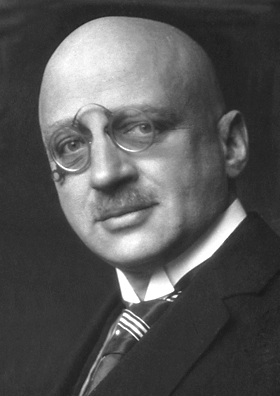
\includegraphics[width=\linewidth]{images/book3/haber.png}
\end{minipage}\hspace{0.01\linewidth}%
\begin{minipage}[t]{0.15\linewidth}\vspace{0pt}
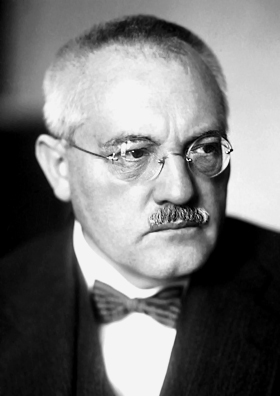
\includegraphics[width=\linewidth]{images/book3/bosch.jpg}
\end{minipage}\hfill
\begin{minipage}[t]{0.66\linewidth}\vspace{0pt}
Fritz Haber (1868--1934) mat het evenwicht van ammoniak onder druk
en liet het in 1909 continu stromen uit een laboratoriumconverter over een
osmiumkatalysator. Carl Bosch (1874--1940) maakte er een industrie van, met
stalen vaten die bestand waren tegen hete waterstof onder druk en een goedkope ijzerkatalysator;
de eerste fabriek startte in 1913. Haber kreeg de Nobelprijs in
1918, Bosch in 1931. (Portretten van de Nobelstichting: publiek domein, Wikimedia
Commons.)
\end{minipage}
\end{history}

\subsection*{Zwaveltrioxide}

In het contactproces verloopt \ce{2SO2(g) + O2(g) <=> 2SO3(g)} ($\Delta_r H^\circ =
\qty{-197.8}{kJ/mol}$ voor de vergelijking zoals geschreven) over een katalysator van
vanadiumoxide, die alleen heet actief is, in verscheidene adiabatische bedden. In elk bed
verhoogt de vrijgekomen warmte de temperatuur, wat $K^\circ$ verlaagt; de omzetting
stopt wanneer het gas de evenwichtskromme bereikt. Afkoelen tussen de bedden brengt
het terug naar een temperatuur waarbij het evenwicht meer omzetting toelaat.
% ledger: dfh:SO2_g, dfh:SO3_g

\begin{omfigure}
\begin{tikzpicture}
\begin{axis}[
  width=0.72\linewidth, height=6.4cm, xmin=600, xmax=900, ymin=0, ymax=1.08,
  axis x line=bottom, axis y line=left, xlabel={$T$ (K)},
  ylabel={omzetting van \ce{SO2}}, tick label style={font=\small},
  label style={font=\small}, clip=false]
\addplot[black, very thick] table[x=T, y=X] {figdata/out/bachelor-2-vant-hoff-c.dat};
\addplot[omThm, thick] table[x=T, y=X] {figdata/out/bachelor-2-vant-hoff-bed1.dat};
\addplot[omThm, thick] table[x=T, y=X] {figdata/out/bachelor-2-vant-hoff-bed2.dat};
\addplot[omThm, thick] table[x=T, y=X] {figdata/out/bachelor-2-vant-hoff-bed3.dat};
\draw[->, omDef, thick] (axis cs:892.8,0.676) -- (axis cs:712,0.676);
\draw[->, omDef, thick] (axis cs:784.4,0.924) -- (axis cs:712,0.924);
\node[font=\scriptsize, anchor=south west] at (axis cs:860,0.84) {evenwicht};
\node[omThm, font=\scriptsize, anchor=west] at (axis cs:800,0.24) {bed 1 (adiabatisch)};
\node[omDef, font=\scriptsize, anchor=south] at (axis cs:800,0.68) {koeling};
\end{axis}
\end{tikzpicture}

{\small Evenwichtsomzetting van \ce{SO2} naar \ce{SO3} als functie van de temperatuur
(zwart) voor een modelvoeding van \qty{10}{\percent} \ce{SO2}, \qty{11}{\percent}
\ce{O2} bij \qty{1}{bar}, en de weg van het gas door drie adiabatische bedden
(rood, stijgend in temperatuur doordat de reactie het gas verwarmt), afgekoeld tussen de
bedden (blauw).}
% ledger: janafG:SO2.600, janafG:SO2.700, janafG:SO2.800, janafG:SO2.900, janafG:SO3.600, janafG:SO3.700, janafG:SO3.800, janafG:SO3.900 (computed in figdata/bachelor-2/vant-hoff.py; feed and adiabatic rise are model values)
\end{omfigure}

\section{Oefeningen}

\begin{exercise}[$\star$]\label{exo:b2:equilibrium-shifts:1}
Bereken $K^\circ$ bij \qty{298}{K} voor een reactie met $\Delta_r G^\circ =
\qty{-32.8}{kJ/mol}$, en daarna voor $\Delta_r G^\circ = \qty{+32.8}{kJ/mol}$.
Welke verandering van $\Delta_r G^\circ$ vermenigvuldigt $K^\circ$ met 100?
\end{exercise}

\begin{exercise}[$\star$]\label{exo:b2:equilibrium-shifts:2}
Voor de ammoniaksynthese is $K^\circ(298) = \num{5.4e5}$ en $\Delta_r H^\circ =
\qty{-91.9}{kJ/mol}$. Schat $K^\circ$ bij \qty{400}{K} met de geïntegreerde
\omterm{thm:b2:equilibrium-shifts:vant-hoff}{vergelijking van Van 't Hoff}; de tabellen geven 35.6.
\end{exercise}

\begin{exercise}[$\star$]\label{exo:b2:equilibrium-shifts:3}
Bereken de \omterm{def:b2:equilibrium-shifts:variance}{variantie} van: (a) vloeibaar water in evenwicht met zijn damp;
(b) \ce{CaCO3(s) <=> CaO(s) + CO2(g)} in een gesloten vat; (c) \ce{N2},
\ce{H2}, \ce{NH3} in evenwicht, willekeurige voeding; (d) \ce{C(s) + H2O(g) <=>
CO(g) + H2(g)}.
\end{exercise}

\begin{exercise}[$\star$]\label{exo:b2:equilibrium-shifts:4}
Voor \ce{N2O4(g) <=> 2NO2(g)} is $\Delta_r H^\circ > 0$. In welke richting verschuift het
evenwicht door verwarmen bij constante druk, door samenpersen bij
constante temperatuur, door argon toe te voegen bij constant volume?
\end{exercise}

\begin{exercise}[$\star\star$]\label{exo:b2:equilibrium-shifts:5}
Voor \ce{N2(g) + O2(g) <=> 2NO(g)} is $\Delta_r H^\circ = \qty{180.6}{kJ/mol}$ en
$\Delta_r S^\circ = \qty{24.8}{J/(K.mol)}$. Bereken $K^\circ$ bij \qty{298}{K}
en bij \qty{2000}{K} (\omterm{def:b2:reaction-free-energy:ellingham-approximation}{benadering van Ellingham}), en de molfractie
\ce{NO} in lucht ($x(\ce{N2}) = 0.78$, $x(\ce{O2}) = 0.21$, weinig verbruikt) bij
evenwicht bij \qty{2000}{K}. Waarom maken motoren deze verontreiniging, en waarom
blijft ze bestaan in de afgekoelde uitlaatgassen?
\end{exercise}

\begin{exercise}[$\star\star$]\label{exo:b2:equilibrium-shifts:6}
Een verestering $\mathrm{A + B \rightleftharpoons E + W}$ in de vloeistoffase
heeft $K^\circ = 4.0$ (activiteiten gelijkgesteld aan molfracties). Bereken, uitgaande van
\qty{1.0}{mol} zuur A, de hoeveelheid ester met \qty{1.0}{mol} en daarna met
\qty{3.0}{mol} alcohol B. Leg met $Q$ en $K^\circ$ uit waarom het verwijderen van het
water naarmate het ontstaat, de reactie tot volledigheid drijft.
\end{exercise}

\begin{exercise}[$\star\star$]\label{exo:b2:equilibrium-shifts:7}
Bij \qty{298}{K} en \qty{1}{bar} is $K^\circ = 0.148$ voor \ce{N2O4 <=> 2NO2}.
Bereken de dissociatiegraad van \qty{1}{mol} \ce{N2O4}. Daarna wordt
\qty{1}{mol} argon toegevoegd bij constante totale druk: bereken de nieuwe
dissociatiegraad, en verklaar. Wat gebeurt er als het argon bij
constant volume wordt toegevoegd?
\end{exercise}

\begin{exercise}[$\star\star$]\label{exo:b2:equilibrium-shifts:8}
Ammoniumchloride sublimeert door te dissociëren, \ce{NH4Cl(s) <=> NH3(g) +
HCl(g)}. Bereken de \omterm{def:b2:equilibrium-shifts:variance}{variantie} wanneer het gas alleen door de vaste stof gevormd wordt, en wanneer
er wat ammoniak is toegevoegd. Wat betekent elk geval voor de experimentator?
\end{exercise}

\begin{exercise}[$\star\star$]\label{exo:b2:equilibrium-shifts:9}
De tabellen geven voor de ammoniaksynthese $K^\circ = 0.0993$ bij \qty{500}{K} en
$K^\circ = \num{1.72e-3}$ bij \qty{600}{K}. Leid daaruit $\Delta_r H^\circ$ in dat
interval af en vergelijk met de waarde bij \qty{298}{K}.
\end{exercise}

\begin{exercise}[$\star\star\star$]\label{exo:b2:equilibrium-shifts:10}
Bewijs het tegenvoorbeeld van \cref{rem:b2:equilibrium-shifts:paradox}: schrijf
$Q$ van de ammoniaksynthese met de hoeveelheden en de totale druk, bereken
$\partial\ln Q/\partial n(\ce{N2})$ bij constante $T$ en $p$, en bepaal de
voorwaarde op $x(\ce{N2})$ waarvoor het toevoegen van stikstof het evenwicht
achterwaarts verschuift. Kan hetzelfde gebeuren bij constant volume?
\end{exercise}

\begin{exercise}[$\star\star\star$]\label{exo:b2:equilibrium-shifts:11}
Kalksteen wordt verhit tot \qty{1100}{K} in een leeg, gesloten vat van
\qty{10.0}{L}, waar $\Delta_r G^\circ = \qty{1.62}{kJ/mol}$ voor zijn
ontleding (\cref{ch:b2:reaction-free-energy}). Bereken $K^\circ$ en de
evenwichtsdruk van koolstofdioxide. Bepaal de eindtoestand voor
\qty{0.050}{mol} en voor \qty{0.200}{mol} kalksteen.
\end{exercise}

\begin{exercise}[$\star\star\star$]\label{exo:b2:equilibrium-shifts:12}
Lees op de figuur van het contactproces de omzetting en de temperatuur af aan de
uitlaat van elk bed. Leg uit waarom één adiabatisch bed, hoe lang ook,
met deze voeding niet boven ongeveer 68\,\% omzetting zou kunnen uitkomen, waarom het gas
tussen de bedden wordt afgekoeld in plaats van de katalysator overal koud te houden, en wat
de omzetting van het laatste bed begrenst.
\end{exercise}

\section{Probleem: de ammoniakkringloop}

\begin{problem}[{Weekendprobleem --- de evenwichtsconstante van de
ammoniaksynthese en haar temperatuurafhankelijkheid, de samenstelling onder de omstandigheden
van de converter, de verschuivingen door druk, temperatuur en inerte gassen, en
de kringloop}]
\label{pb:b2:equilibrium-shifts:1}
Ammoniak wordt gemaakt volgens \ce{N2(g) + 3H2(g) <=> 2NH3(g)} uit een stoichiometrische voeding.
Gegevens: bij \qty{298.15}{K} is $\Delta_f H^\circ(\ce{NH3}) = \qty{-45.94}{kJ/mol}$,
$S^\circ_m$ (\unit{J/(K.mol)}) \ce{NH3} 192.77, \ce{N2} 191.61, \ce{H2} 130.68;
de tabellen geven $\Delta_f G^\circ(\ce{NH3}) = \qty{+27.19}{kJ/mol}$ bij
\qty{700}{K} en \qty{+38.66}{kJ/mol} bij \qty{800}{K}. De gassen zijn ideaal;
$R = \qty{8.314}{J/(K.mol)}$.
% ledger: dfh:NH3_g, s0:NH3_g, s0:N2_g, s0:H2_g, janafG:NH3.700, janafG:NH3.800

\medskip
\noindent\textbf{Deel I --- De constante.}
\begin{enumerate}
  \item Bereken $\Delta_r H^\circ$, $\Delta_r S^\circ$ en $\Delta_r G^\circ$ bij
        \qty{298}{K}, en $K^\circ(298)$.
  \item Bereken $K^\circ$ bij \qty{700}{K} en bij \qty{800}{K} uit de tabellen.
  \item Leid uit deze twee waarden de gemiddelde $\Delta_r H^\circ$ af tussen
        \qty{700}{K} en \qty{800}{K}, en vergelijk met vraag 1.
  \item Schat $K^\circ(\qty{723}{K})$ uit de twee getabelleerde waarden met
        de \omterm{thm:b2:equilibrium-shifts:vant-hoff}{vergelijking van Van 't Hoff}.
  \item Bereken $K^\circ(\qty{723}{K})$ in de \omterm{def:b2:reaction-free-energy:ellingham-approximation}{benadering van Ellingham} uit
        de gegevens bij \qty{298}{K}, en becommentarieer het verschil.
\end{enumerate}

\medskip
\noindent\textbf{Deel II --- Het evenwicht in de converter.}
\begin{enumerate}[resume]
  \item Schrijf, uitgaande van een voeding van \qty{1}{mol} \ce{N2} en \qty{3}{mol} \ce{H2}, de
        hoeveelheden bij voortgang $\xi$ en de totale hoeveelheid op.
  \item Toon aan dat, met $x$ de molfractie ammoniak, de molfracties
        van \ce{N2} en \ce{H2} gelijk zijn aan $(1-x)/4$ en $3(1-x)/4$.
  \item Toon aan dat $\dfrac{x}{(1-x)^2} = \dfrac{\sqrt{27}}{16}\,\dfrac{p}{p^\circ}\,
        \sqrt{K^\circ}$.
  \item Bereken $x$ bij \qty{723}{K} en \qty{1}{bar}.
  \item Bereken $x$ bij \qty{723}{K} en \qty{200}{bar}.
  \item Bereken de \omterm{def:b2:equilibrium-shifts:variance}{variantie} van het systeem en leg uit waarom $T$ en $p$ de
        samenstelling vastleggen.
\end{enumerate}

\medskip
\noindent\textbf{Deel III --- Verschuivingen.}
\begin{enumerate}[resume]
  \item In welke richting verschuift het evenwicht, zonder te rekenen, wanneer
        de druk stijgt? Wanneer de temperatuur stijgt?
  \item Argon komt binnen met de lucht die gebruikt wordt om de stikstof te maken. Hoe verschuift
        zijn aanwezigheid het evenwicht bij constante totale druk?
  \item Een mengsel in evenwicht heeft $x(\ce{N2}) = 0.30$. Verschuift een beetje
        extra stikstof bij constante $T$ en $p$ het evenwicht voorwaarts of achterwaarts?
  \item Zou het antwoord bij constant volume anders zijn?
  \item Voordat het gas naar de converter terugkeert, wordt de ammoniak eruit
        gecondenseerd. Wat doet dat met $Q$ aan de inlaat van de converter?
\end{enumerate}

\medskip
\noindent\textbf{Deel IV --- De kringloop.}
\begin{enumerate}[resume]
  \item Het gas verlaat de converter met \qty{18}{\percent} ammoniak, onder
        de evenwichtswaarde. Waarom bereikt een echte converter het evenwicht
        niet?
  \item Bereken de \omterm{def:b2:equilibrium-shifts:single-pass}{conversie per doorgang} van waterstof die overeenkomt met
        $x(\ce{NH3}) = 0.18$ uit een stoichiometrische voeding.
  \item Het niet-omgezette gas wordt teruggevoerd. In stationaire werking komt per tijdseenheid
        \qty{1.00}{mol} verse \ce{N2} binnen: hoeveel ammoniak gaat er naar buiten, en hoeveel
        stikstof passeert per tijdseenheid door de converter?
  \item Waarom moet er een beetje gas uit de \omterm{def:b2:equilibrium-shifts:single-pass}{recyclestroom} gespuid worden?
  \item Waarom laat men de converter niet bij \qty{500}{K} werken, waar het evenwicht
        veel gunstiger is?
  \item Geef de molfractie ammoniak bij evenwicht bij \qty{723}{K} en
        \qty{200}{bar} voor een stoichiometrische voeding, in het model van de ideale gassen.
\end{enumerate}
\end{problem}
